\documentclass[a4paper]{extbook}
\usepackage[russian]{babel} 
\usepackage[utf8]{inputenc} 
\usepackage[T2A]{fontenc} 
\usepackage{cslav,color,pscyr,geometry,psfrag,graphicx,xcolor,epigraph,ifthen} 
\showboxdepth=\maxdimen
\showboxbreadth=\maxdimen

\usepackage[
contents={},
opacity=1,
scale=1.5,
color=black
]{background}

\AddEverypageHook{%
{\ifthenelse{\thepage=1}{\backgroundsetup{contents={}}}%
{\ifthenelse{\isodd{\value{page}}}%
{\backgroundsetup{
angle=0,
position={10.4cm,-8.122cm},
contents={\rule{2.2pt}{14cm}}
}%
}%
{\backgroundsetup{
angle=0,
position={0.225cm,-8.122cm},%
contents={\rule{1.9pt}{14cm}}
}%
}%
\BgMaterial}}}


\graphicspath{{illustrations/}}
\makeatletter
\renewcommand{\@evenhead}{\vbox {\vspace*{-1.2cm}\hbox to \textwidth%
    {\hfil \fontfamily{agrr}\selectfont{\Large -- {Orgy of The Righteous}    -- } \hfil\strut} \vspace*{-1.3cm}\hbox to 0pt%
{\hspace*{-2.2cm}
\includegraphics[width=3cm]{./borders/even.eps}}%
{\vspace*{-1.615cm}\hspace*{0.6cm}\rule{17cm}{2.3pt}} 
}}
\renewcommand{\@oddhead}{\vbox {\vspace*{-1.2cm}\hbox to \textwidth%
    {\hfil \fontfamily{agrr}\selectfont{\Large -- {Orgy of The Righteous}    -- } \hfil\strut} \vspace*{-1.3cm}\hbox to 0pt%
{\hspace*{14.2cm}
\includegraphics[width=3cm]{./borders/odd.eps}}%
{\vspace*{-1.615cm}\hspace*{-2.6cm}\rule{17cm}{2.3pt}} 
}}
\renewcommand{\@evenfoot}{\vbox { \vspace*{0.7cm}\hbox to 0pt%
{\hspace*{-2.2cm}
\includegraphics[width=3cm]{./borders/evenfoot.eps}}%
{\vspace*{-2.32cm}\hspace*{0.6cm}\rule{17cm}{2.3pt}} \hbox to \textwidth%
{\hfil \fontfamily{agrr}\selectfont{\LARGE -- {\thepage}    -- } \hfil}
}}
\renewcommand{\@oddfoot}{\vbox { \vspace*{0.7cm}\hbox to 0pt%
{\hspace*{14.2cm}
\includegraphics[width=3cm]{./borders/oddfoot.eps}}%
{\vspace*{-2.32cm}\hspace*{-2.6cm}\rule{17cm}{2.3pt}} \hbox to \textwidth%
{\hfil \fontfamily{agrr}\selectfont{\LARGE -- {\thepage}    -- } \hfil}
}}
\makeatother

\newcommand{\dropcamred}[1] {
  {\csl\center\fontfamily{bukv}\fontshape{indycton}\selectfont\cslfsize{200}{}\color{red}#1}}  
  \newcommand{\dropcamredsmall}[1] {
  {\csl\center\fontfamily{bukv}\fontshape{indycton}\selectfont\cslfsize{100}{}\color{red}#1}}  
\newcommand{\dropcamblue}[1] {
  {\csl\center\fontfamily{bukv}\fontshape{indycton}\selectfont\cslfsize{200}{}\color{blue}#1}}  
  
\newcommand{\firstcam}[2] {
\begin{center} \fontfamily{fac}\selectfont{{ \Huge\color{red}#1}{\LARGE#2}}\end{center}\normalfont
}
  
\newcommand{\midcam}[3] {
\begin{center} \fontfamily{fac}\selectfont{{\LARGE#1}{\Huge\color{red}#2}{\LARGE#3}}\end{center}\normalfont
}
 
 
\newcommand{\atendcam}[2] {
\begin{center} \fontfamily{fac}\selectfont{{ \LARGE#1}{\Huge\color{red}#2}}\end{center}\normalfont
}
\setlength{\epigraphwidth}{0.52\textwidth}
\begin{document}
\begin{titlepage}
Это просто титульный лист. 
Тут можно что-то написать, всякие там штуки, типа названия, благодарностей, матерных частушек, нарисовать бобра и всё такое, но сейчас он нужен, чтобы не возникало путаницы между четными и нечетными страницами(обычно четные находятся слева, а нечетные справа)
\end{titlepage}
\begin{figure}[h]
\center{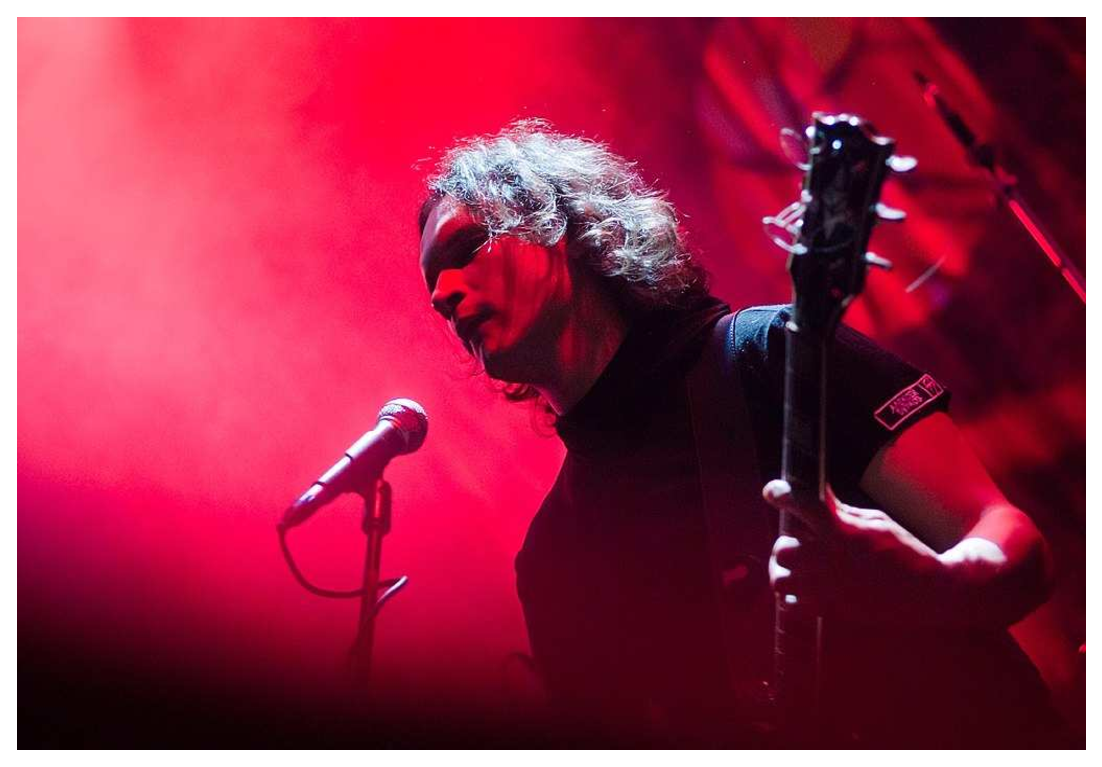
\includegraphics[width=1\linewidth]{a.eps}}
\end{figure}
\firstcam{А}{лексей Николаевич Бурков}

\epigraph{Настоящая музыка пишется, когда ты на ощупь идешь в неизведанное.}{Алексей Бурков}

 Альфа и Омега Оргии Праведников. С самого первого альбома стоит у руля группы, твердой рукой прокладывая курс  в светлое будущее.
Кудесник электрогитары, художник звука, мастер на все руки, отец-герой.

Поклонник Шнитке, King Crimson, Кино, Металлики, что на выходе дает ревущую мелодичность, которая и отличает Оргию Праведников от остальных, либо ревущих, либо мелодичных.
\begin{verse}
Алексей про… \\
…музыку: «\emph{Я считаю что музыка – эта некая нематериальная пилюля, которую человек проглатывает, а потом становится другим. Собственно это можно сказать про любое искусство.}»\\
…страхи: «\emph{Больше всего я боюсь перестать слышать Музыку. Вот я хожу, живу, и откуда-то оттуда слышу Музыку. А вот если я её однажды не услышу – это и есть самое страшное}». \\
\end{verse}


\begin{figure}[h]
\center{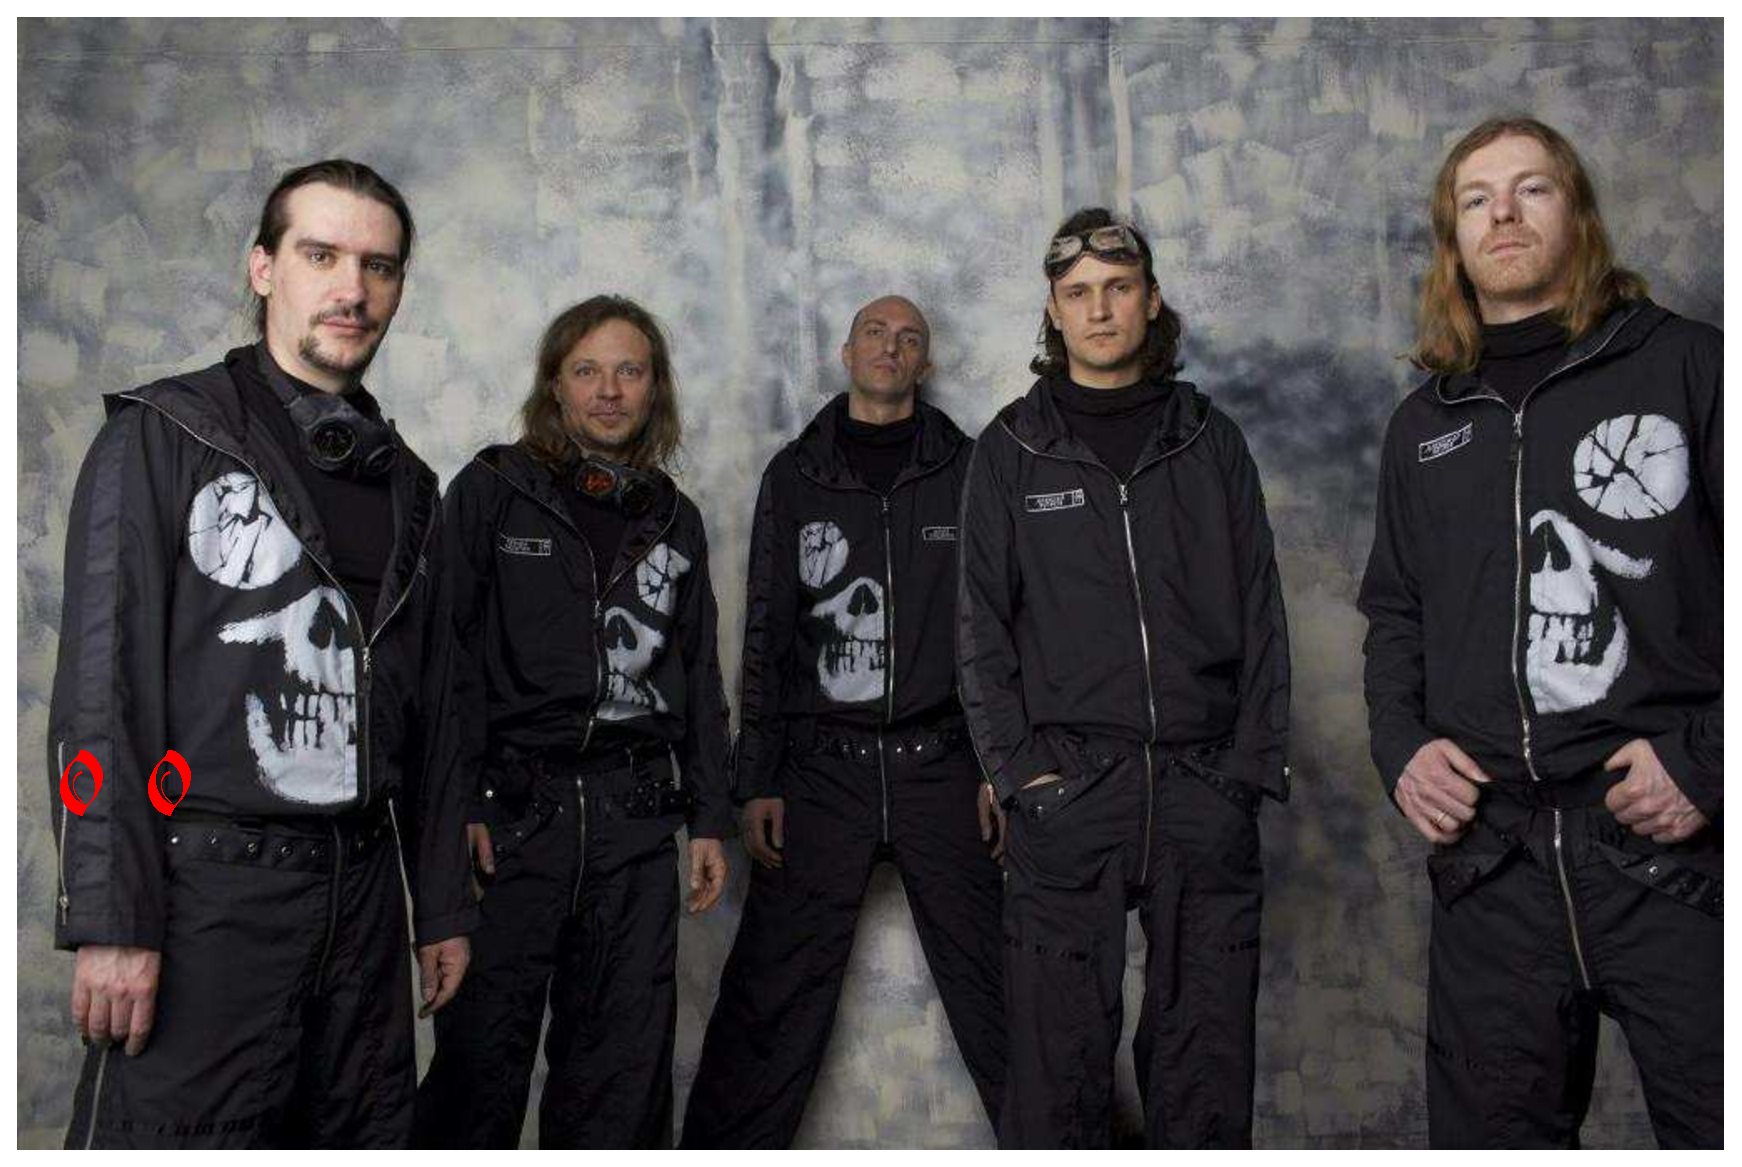
\includegraphics[width=1\linewidth]{yo.eps}}
\end{figure}
\midcam{Од}{Ё}{жа}
\epigraph{Я еле-еле поднимаюсь, в темноте ищу штаны \\ Отбросив кресло, понимаю, что штаны не так важны}{Сергей Калугин}
 
Давным-давно, когда на обложках альбомов не было даже фамилий музыкантов, на сцену они выходили в чем попало. Попадало по-всякому и не всегда удачно.

Но настал момент, когда за группу железной рукой взялись Татьяна Буркова и ее фирма "Касталан". И с того самого момента, следуя завету классика, в человеке буквально всё стало прекрасно: и лицо, и одежда, и всё остальное.

А после того, как с недавних пор к процессу подключилась Елизавета Сорочинская, сценические образы достигли прямо-таки неописуемой красоты.


Однако одеждой для музыкантов дело не ограничивается! Обо всех нас "Касталан" заботится не хуже родной мамы: футболки и толстовки, кепки и банданы, шарфы и даже тапки – поклонник Оргии одет практически с головы до ног. И только такая важная деталь, как штаны, пока не нашла себе места в реестре оргиевского мерча. Как видно, фирма следует завету другого классика, который поведал нам, что "штаны не так важны". Ну и ладно.
 
 \begin{figure}[h]
\center{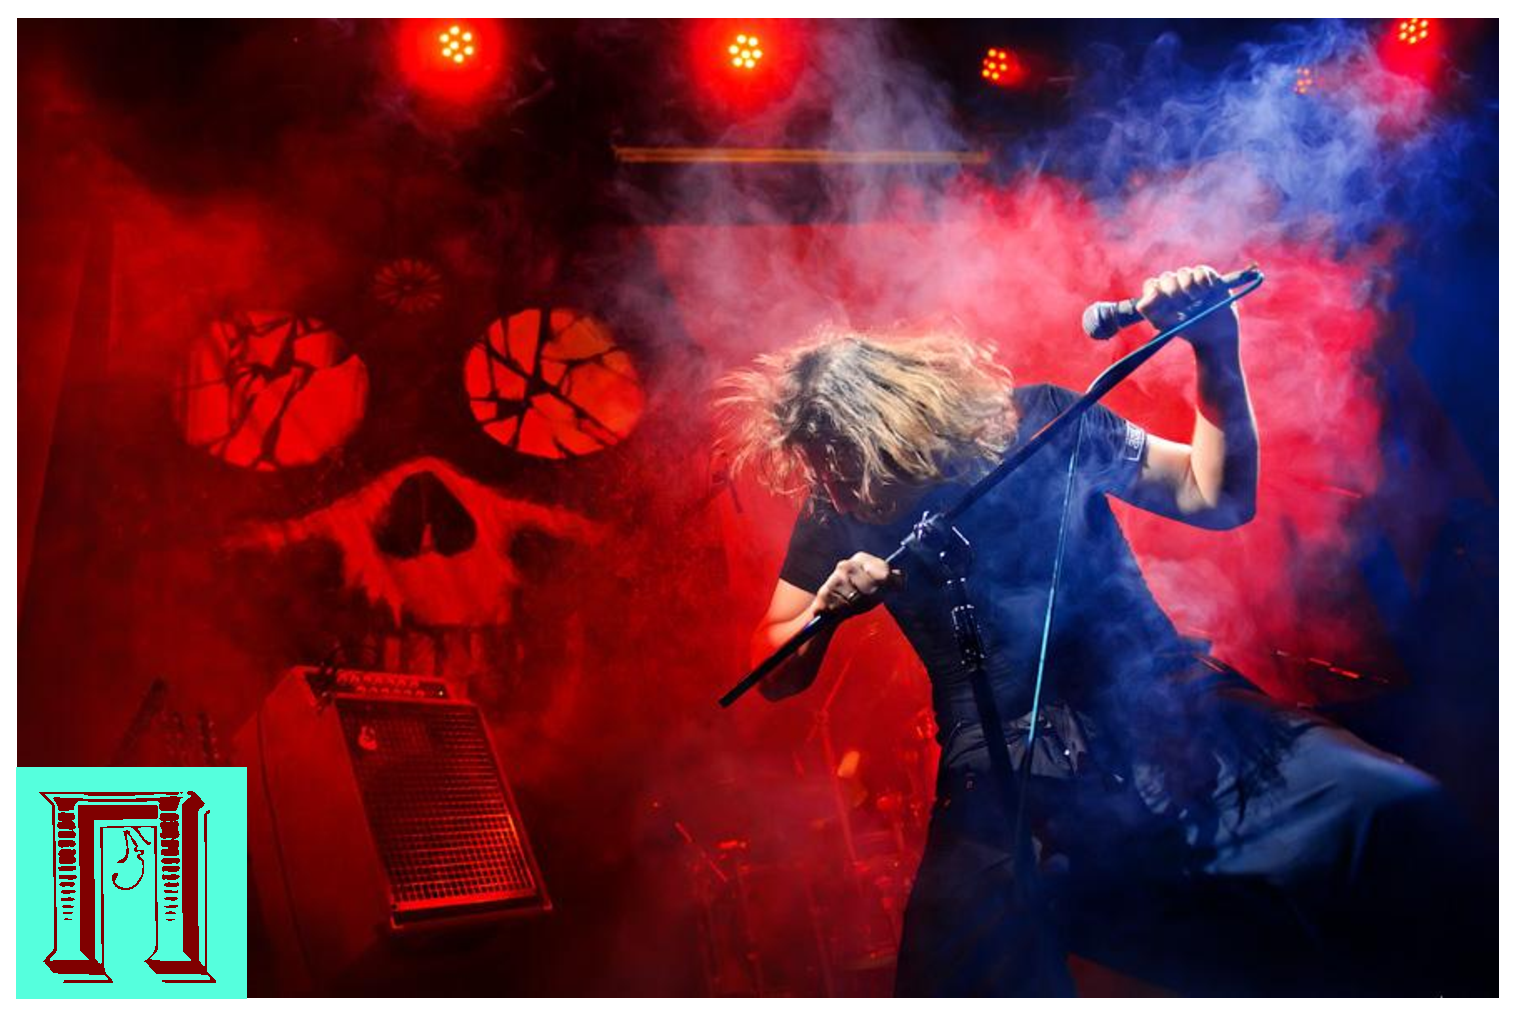
\includegraphics[width=1\linewidth]{p.eps}}
\end{figure}
\firstcam{П}{оздно делать тише}
\setlength{\epigraphwidth}{0.4\textwidth}
\epigraph{Ну, и что вы споёте теперь, \\
Вечно голодные толпы и слуги народа?}{Сергей Калугин, "Радио Армагеддон"}
 Гениальная фраза, произнесённая звукорежиссёром Ильёй во время одного из выступлений в Днепропетровске.

"\emph{Илья был парень зело рукастый и ушастый, по части звука смекалистый. Внешность имел самую что ни на есть иисусоподобную: худенький, круглолицый, длинноволосый и усатенький, очень благостный и сероглазый. Достать, разозлить Илью было весьма проблематично, но все же был один простой способ: приставать к нему, когда он чудодействовал над пультом}".

Фраза была произнесена с должной экспрессией в тот самый момент, когда некие "солидные сеньоры" из первого ряда внезапно для себя открыли, что рок-концерт(а уж тем более концерт "Оргии"), оказывается, далеко не самое тихое и привычное для их ушей священнодейство. 

В последствии это самое "Поздно делать тише" надолго вошло в обиход как у группы, так и у её поклонников. 

 
\end{document}